\setcounter{chapter}{-1}
\notocchapter{Prologue}
%
\vspace{-\onelineskip}
\fancyquote{Ralph Waldo Emerson}%
{The sea, washing the equator and the poles, offers its perilous aid, and the power and empire that follow it [...]. \enquote{Beware of me}, it says, \enquote{but if you can hold me, I am the key to all the lands}.}
\vspace{\onelineskip}

Cross-equatorial flow has a major influence on the World's climate. It effectively couples both the northern and southern hemisphere in latitude, but also the Atlantic, Pacific and Indian Oceans in longitude, exchanging heat and matter between regions that lie thousands of kilometers apart. Equatorial processes like the \acf{ENSO} influence countless human lives, \eg through the extreme weather events observed during \emph{El Ni\~{n}o} (\figref{fig:fire-indonesia}). Another example is the \acf{AMOC} and the resulting Gulf Stream, which is the reason for the mild European climate compared to that of \eg the East Coast of North America.

However, despite its crucial role in understanding our climate, cross-equatorial flow is still not very well researched.
The absence of a Coriolis parameter at \ang{0} latitude makes it impossible to apply geostrophic balance or other leading-order approximations, so the dynamics in the equatorial region are determined by processes that are hard to quantify like nonlinearity and friction (\cite{pedloskyoct}; \cite{edwards}).

While many studies focus on either the driving processes of the \ac{MOC} and thus the forcing of cross-equatorial flow (\cite{kuhlbrodt}; \cite{marshall}), or the mechanics of cross-equatorial flow with a fixed inter-hemispheric forcing (such as \cite{edwards}; \cite{kawase}), the kinematic processes involved in \emph{enabling} cross-equatorial flow are less well studied. Due to the success of simple models such as the Stommel box model \citep{stommelbox} or the Stommel-Arons model \citep{stommel-arons}, a cross-hemispheric pressure gradient is often implicitly assumed to result in a cross-equatorial flow, without paying attention to the actual dynamics at the equator.

An interesting study is found in \cite{killworth}, which examines cross\hyp{}equatorial geostrophic adjustment, \ie an unforced spin-up after a mass imbalance between the hemispheres has been released\sidenote[-2]{For more information on the \citeauthor{killworth} model refer to \secref{sec:killworth}.}. Using his equatorial shallow-water model, \citeauthor{killworth} proceeds to show that in an inviscid, one-dimensional ocean, water may at most penetrate about two Rossby radii of deformation into the opposite hemisphere. After extending his model to a two-dimensional basin and introducing lateral friction, \citeauthor{killworth} found that transport to high latitudes of the opposite hemisphere is now possible, enabled by friction that acts to dissipate excessive \emph{\ac{PV}} (\secref{sec:general-vorticity}). At the same time, \citeauthor{killworth} found a lower interior transport across the equator when lowering the lateral diffusivity (here referred to as viscosity).

Since the Earth's ecosystem offers a sheer infinite level of complexity, there is only so much insight one may gain from observations and analytical solutions. One immensely valuable tool in understanding our climate are \acp{GCM}, which are becoming more powerful each day as research in modeling and computational sciences progresses. However, despite their usefulness, error margins are often large due to uncertainties in initial conditions (from observations), parameters, parameterizations, or even the physical processes itself. 

Some of these uncertainties are caused by the parameterization of friction in climate models, which is usually not based on first principles but, on the contrary, treated rather heuristically\sidenote[-2]{\Cf \secref{sec:physics-friction}.}. Often, unrealistically high viscosities are assumed in order to suppress numerical noise (\secref{sec:noise}), since diffusive friction leads to smoother numerical solutions. However, lowering viscosity and accepting some noise in the solution may in fact lead to physically more relevant solutions, as shown in \eg \cite{jochum}.

That being said, the question I set out to answer in this thesis can be formulated as:

{\slshape
How sensitive is the meridional overturning in low-resolution simulations towards changes in lateral diffusivity, and thus the magnitude of friction that is acting at the equator?
}

In particular, since it is known that friction is crucial in enabling cross-equatorial flow through the transformation of potential vorticity (\secref{sec:equatorial-theory}), to what extent is it possible to control the magnitude of the overturning through viscosity modifications in \ac{CESM}, a state-of-the-art climate model, and what is suggested by theory?

\begin{figure}[b!]
	\begin{sidecaption}[Smoke above Indonesia during the 2016 wildfires.]{Smoke above Indonesia, released during the 2016 wildfires, which are amplified by El Ni\~{n}o. Satellite image by \href{http://http://www.nasa.gov/feature/goddard/2016/el-nino-brought-drought-and-fire-to-indonesia}{NASA}.}[fig:fire-indonesia]
		\antimpjustification
		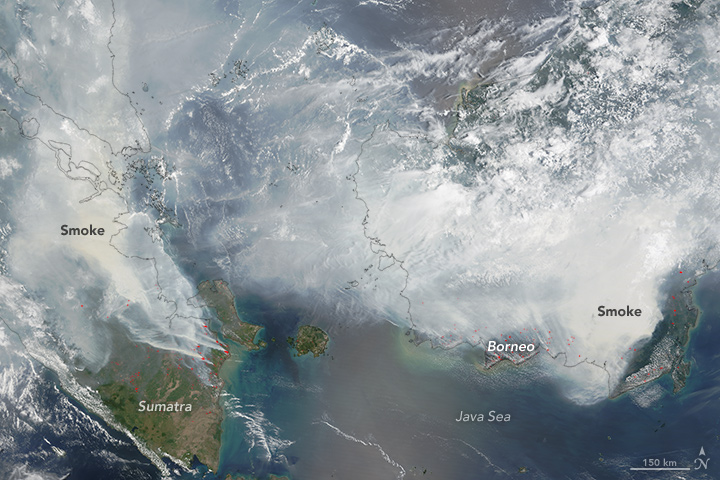
\includegraphics[width=.85\textwidth]{preface/wildfires}
	\end{sidecaption}
\end{figure}